% created by Sebastian Nemak - der-basti.com
\documentclass[
	12pt % default font size
	,a4paper % classic A4 page, default onesided
	,BCOR=12mm % binding correction
	,headings=normal % smarter headings
	,toc=graduated % table of content (toc) with indent (not '=flat')
	,bibliography=totoc % toc bibliography
]{scrreprt} % KOMA-Script report document typ

% -----------------------------------------------------------------------------
% packages, settings, \renewcommand and meta data
% -----------------------------------------------------------------------------

\usepackage[utf8]{inputenc} % set utf-8 input encoding
\usepackage[T1]{fontenc} % 8-bit encoding for languages with accented characters
\usepackage[ngerman,english]{babel} % to use (new) german and english language
\usepackage{lmodern} % use vector font
\usepackage[top=3cm, right=25mm, bottom=3cm, headsep=1em, footskip=12mm]{geometry}
\usepackage{hyperref} % han­dle cross-ref­er­enc­ing
\usepackage{amsmath,amsfonts,amssymb} % pro­vides math­e­mat­i­cal fea­tures
\usepackage{setspace} % set­ting the spac­ing be­tween lines
\usepackage[german=swiss]{csquotes} % pro­vides ad­vanced fa­cil­i­ties for in­line and dis­play quo­ta­tions e.g. \enquote{Text}
\usepackage{graphicx} % grafic
\usepackage[printonlyused]{acronym} % import package and print only used acronyms
\usepackage{harvard} % har­vard ci­ta­tion style with sev­eral vari­ant styles
\usepackage[automark,headsepline]{scrlayer-scrpage} % for header and footer
\usepackage{scrhack,listings} % package for source code listings %TODO ,filecontents for line numbers
	\usepackage[usenames,dvipsnames]{color} % for syntax highlighting

\usepackage{blindtext} % OPTINAL: for demo text purposes

\hypersetup{ % pdf options
	pdfauthor = {Your Name}
	,pdftitle = {Latex Template}
	,pdfsubject = {bachelor or master thesis subject}
	,pdfcreator = {\LaTeX}
	,pdfkeywords = {Stichwort1, Stichwort2 ...}
	,pdfproducer = {pdfTeX \the\pdftexversion.\pdftexrevision}
	,breaklinks=true,unicode=false, pdftoolbar=true, pdfmenubar=true, pdffitwindow=false, pdfstartview={FitH},pdfnewwindow=true
	,colorlinks=true, linkcolor=black, citecolor=black, filecolor=magenta, urlcolor=black
}
\setcounter{tocdepth}{3} % toc depth level - list subsubsection
\setcounter{secnumdepth}{3} % toc depth level - number subsubsection
\setlength\parindent{0pt} % 0/no auto paragraph indent
\graphicspath{ {images/}{screenshots/} } % grafic - set basic directories
\DeclareGraphicsExtensions{.pdf,.png,.jpg,.jpeg,.gif,.tif,.tiff} % grafic - default file extensions
% header and footer settings
	\clearpairofpagestyles
	\cfoot[\pagemark]{\pagemark}
	\pagestyle{scrheadings}
% color source code listings
\lstset{ %TODO language=Java,
	breaklines=true
	,captionpos=b
	,numbers=left
	,basicstyle=\ttfamily\scriptsize
	,keywordstyle=\color{blue}\ttfamily
	,stringstyle=\color{red}\ttfamily
	,commentstyle=\color{ForestGreen}\ttfamily
	,morecomment=[l][\color{magenta}]{\#}
}

\author{Your Name}
\title{Latex Template}
\subtitle{bachelor or master thesis subject}
\date{\today}

\begin{document}

\selectlanguage{ngerman}

% Vorspann
\renewcommand{\thesection}{\Roman{section}} \renewcommand{\theHsection}{\Roman{section}}
\pagenumbering{Roman}

% -----------------------------------------------------------------------------
% title page
% -----------------------------------------------------------------------------

\maketitle

% -----------------------------------------------------------------------------
% declaration of originality
% -----------------------------------------------------------------------------

\vspace*{1em}
\section*{Erklärung}\rohead{Erklärung}

Hiermit erkläre ich, dass ich die vorliegende Arbeit selbständig angefertigt habe. Es wurden nur die in der Arbeit ausdrücklich benannten Quellen und Hilfsmittel benutzt. Wörtlich oder sinngemäß übernommenes Gedankengut habe ich als solches kenntlich gemacht.\par
\vspace*{2em}
\begin{table}[ht]
	\centering
	\begin{tabular}{ p{6cm} c }
		\underline{Berlin, \today} & \underline{\hspace{5cm}}\\
		Ort, Datum & Unterschrift\\
	\end{tabular}
\end{table}

\pagebreak

% -----------------------------------------------------------------------------
% acknowledgments
% -----------------------------------------------------------------------------

\vspace*{1em}
\section*{Danksagung}\rohead{Danksagung}

Für die Unterstützung ...\par

\pagebreak

% -----------------------------------------------------------------------------
% abstract
% -----------------------------------------------------------------------------

\vspace*{1em}
\section*{Kurzfassung} % use section to print de and en on one page
\addcontentsline{toc}{chapter}{Kurzfassung}
\rohead{Kurzfassung}

\blindtext

\section*{Abstract}
\selectlanguage{english}

\blindtext

\selectlanguage{ngerman}

\newpage

% -----------------------------------------------------------------------------
% table of ...
% -----------------------------------------------------------------------------

\rohead{\headmark} % set header information

\tableofcontents

\pagebreak

\addcontentsline{toc}{chapter}{Abbildungsverzeichnis}
\listoffigures

\pagebreak

\addcontentsline{toc}{chapter}{Tabellenverzeichnis}
\listoftables

\pagebreak

\chapter*{Abkürzungsverzeichnis}
\addcontentsline{toc}{chapter}{Abkürzungsverzeichnis}

\begin{acronym}[Abk.] % longest acronym for indent
	\acro{Abk.}{Abkürzung}
	\acro{z.B.}{zum Beispiel}
	\acro{EU}{Europäischen Union}
	\acro{US}{United States}
	\acro{CN}{China}
	\acro{RU}{Russland}
	\acro{IN}{Indien}
\end{acronym}

\newpage
\onehalfspacing % for the rest document
\renewcommand{\thesection}{\arabic{section}}
\renewcommand{\theHsection}{\arabic{section}}
\pagenumbering{arabic}
\setcounter{section}{0}
\setcounter{page}{1}

% -----------------------------------------------------------------------------
% your content
% -----------------------------------------------------------------------------


\blinddocument

\chapter{Mathematische Formeln}\label{cha:mathematischeFormeln}

\blindmathpaper

\chapter{Formatierungen}\label{cha:formatierungen}

\blindtext

\section{Text}\label{sec:text}

Zum guten Style gehört:
\begin{itemize}
	\item Versuche alle Warnungen beim erstellen zu beheben
	\item Zu einem Chapter, Section, Grafik, Tabelle, ... gehört immer ein \textit{caption} und \textit{label}
\end{itemize}

Umlaute können einfach benutzt werden z.B. äÖü. Hingegen mu{\ss} das {\ss} mit \textbackslash ss umschrieben werden.\par

Text: \textbf{Bold}, \textit{italic}, \emph{Emphasis}.\par

\subsection{Verweise}\label{ssec:verweise}

Referenz: ref: \ref{tab:matrix}, autoref: \autoref{tab:matrix}\par

Fußnote \footnote{Text in der Fußnote}.\par

\enquote{Dies ist ein Zitat direkt in der Zeile.}\par

Eine klassische URL \url{https://google.com}. % url syntax is a little bit different between package hyperref and url
Natürlich kann eine URL auch so aussehen \href{https://google.com}{Google}.\par

Nicht verwendete \ac{Abk.}en werden auch nicht im Verzeichnis aufgenommen. Der Text kann auch \ac{Abk.} enthalten. Folgende Variationen sind möglich.\par
ac: \ac{EU}\par
acs: \acs{EU}\par
acf: \acf{EU}\par
acl: \acl{EU}\par

\subsubsection{Zitation}\label{sssec:citation}

Ein Buch \cite{b:buch}\par
Ein Buch mit Seitenabgabe \cite[S. 3ff.]{b:latex}\par
Ein Buch mit mehreren Authoren \cite{b:komascript}\par
Eine Webreferenz \cite{w:website}\par
Eine längere Zitation.\par
\begin{quote}
	The major improvement concerns the structure of the interview
	(Ulrich~\& Trumbo~1965, p.~112) \ldots \par
	\blindtext
\end{quote}

\begin{verbatim}
	The \BibTeX\ and \LaTeX\ \ldots
\end{verbatim}

\subsection{Ausrichtung}\label{ssec:ausrichtung}

\begin{flushleft}
left
\end{flushleft}

\begin{center}
center
\end{center}

\begin{flushright}
right
\end{flushright}

\subsection{Grö{\ss}en}\label{ssec:groessen}

\begin{tiny}
• tiny
\end{tiny}

\begin{scriptsize}
• scriptsize
\end{scriptsize}

\begin{footnotesize}
• footnotesize
\end{footnotesize}

\begin{small}
• small
\end{small}

\begin{normalsize}
• normalsize
\end{normalsize}

\begin{large}
• large
\end{large}

\begin{Large}
• Large
\end{Large}

\begin{LARGE}
• LARGE
\end{LARGE}

\begin{huge}
• huge
\end{huge}

\begin{Huge}
• Huge
\end{Huge}

\section{Tabellen}\label{sec:tabellen}

\begin{table}[ht]
	\centering
	\label{tab:matrix}
	\begin{tabular}{ | l | c | r | p{5cm} | }
		\hline
		\textbf{Left (l)} & \textbf{Center (c)} & \textbf{Right (r)} & \textbf{p 5cm breit}\\
		\hline
		1 & 2 & 3 & 4\\
		\hline
		5 & 6 & 7 & 8\\
		\hline
	\end{tabular}
	\captionbelow{Matrix Beschriftung}
\end{table}

\section{Grafiken}\label{sec:grafiken}

Um eine Grafik einzufügen benötigt man hier grundsätzlich nur den Dateinamen. Es wird automatisch nach der Datei in den Ordnern \textit{images} und \textit{screenshots} nachgeschlagen. Die zulässigen Dateierweiterungen sind \textit{.pdf}, \textit{.png}, \textit{.jpg}, \textit{.jpeg}, \textit{.gif}, \textit{.tif}, \textit{.tiff}.\par

Das folgende Grafik ist herunter skaliert, da sie für die A4 Seite zu breit ist und somit eine overfull Warnung erzeugt. Demzufolge kann \textit{[scale=0.5]} entfallen.\par

\begin{figure}[ht]
	\centering
	\includegraphics[scale=0.5]{th-wildau-logo_500px-breit}
	\captionbelow{Logo der TH-Wildau auf 0.5 skaliert}
	\label{fig:thWildau050}
\end{figure}

\begin{figure}[ht]
	\centering
	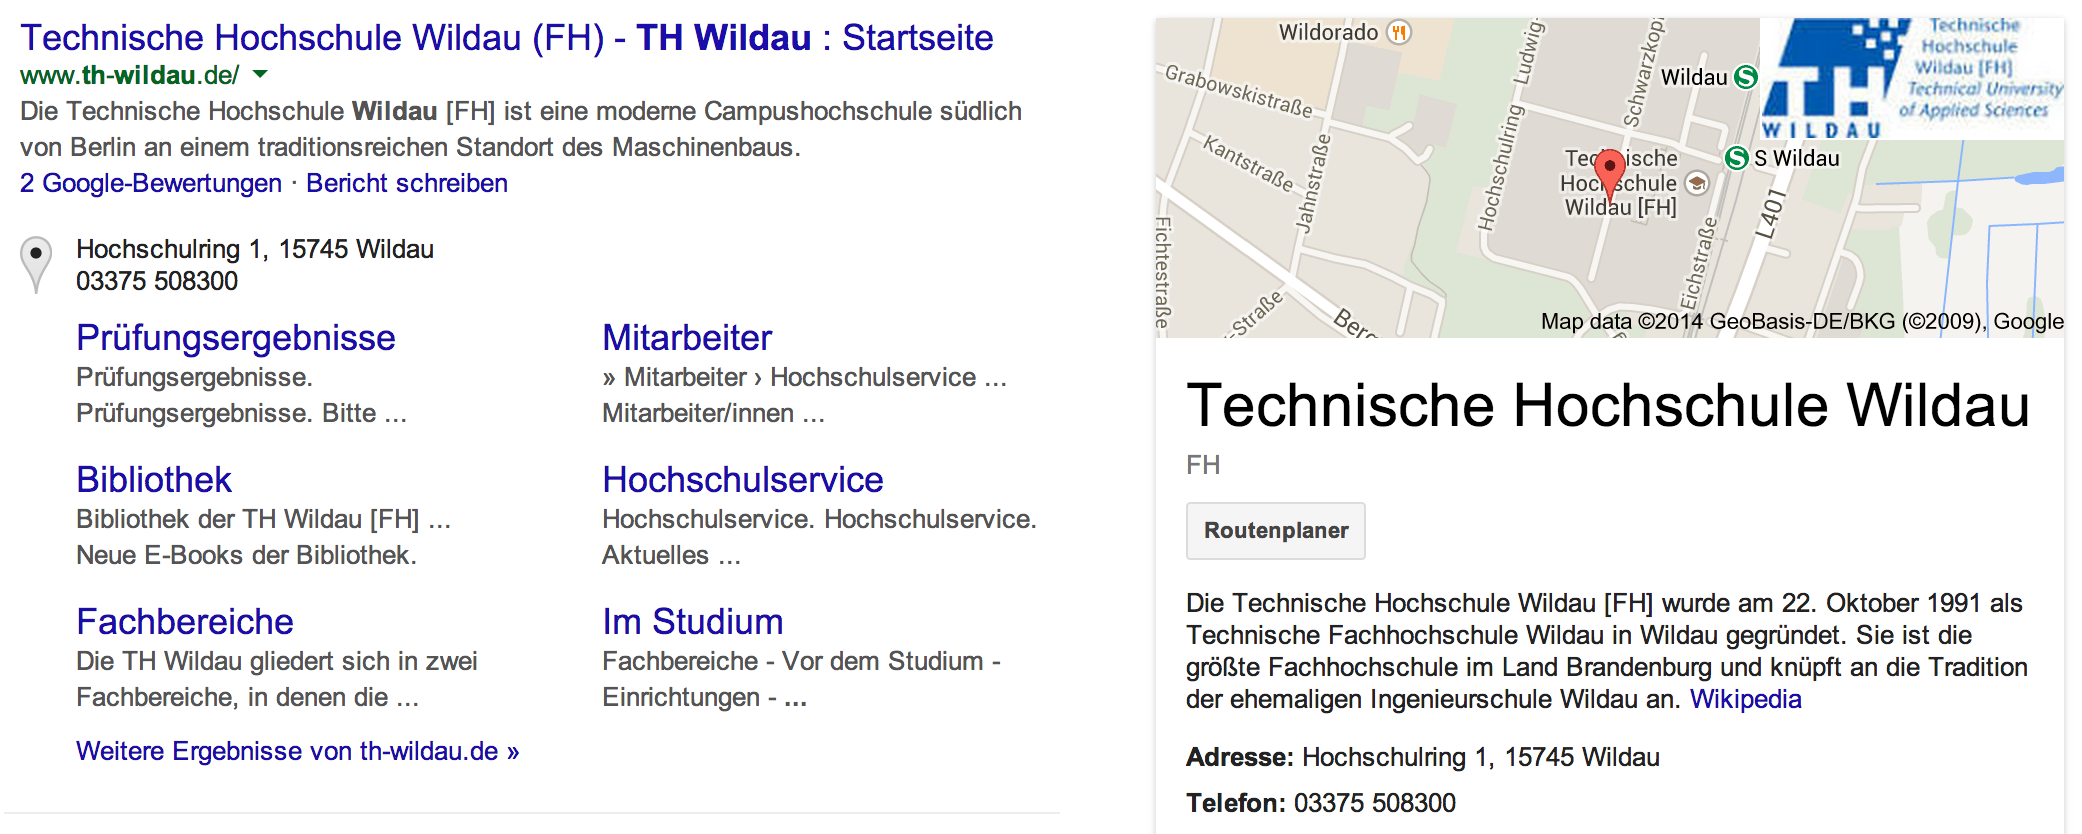
\includegraphics[scale=0.4]{google-q-th-wildau-2014-05-26}
	\captionbelow{Screenshot von Google-Suche nach TH-Wildau am 2014-05-26}
	\label{fig:googleThWildau}
\end{figure}

\subsection{Quellcode}\label{quellcode}

%TODO
 % located here ./thesis.content.sample.tex

\clearpage
\pagebreak
\newpage

% -----------------------------------------------------------------------------
% bibliography
% -----------------------------------------------------------------------------

\bibliographystyle{agsm}
\bibliography{bibo}

% -----------------------------------------------------------------------------
% appendix
% -----------------------------------------------------------------------------

\appendix
\chapter{Appendix}\label{cha:appendix}
\pagenumbering{Roman}
\setcounter{page}{1}

\section*{This section appendix are not listed in the toc}\label{sec:appendixNotInToc}
\section{First appendix}\label{sec:firstAppendix}

\newpage

\section{Second appendix}\label{sec:secondAppendix}

\end{document}